\documentclass[12pt,twoside]{report}
\usepackage{tikz}
\usetikzlibrary{positioning, fit, arrows.meta}
\usepackage{amsmath,amssymb}

%%%%%%%%%%%%%%%%%%%%%%%%%%%%%%%%%%%%%%%%%%%%%%%%%%%%%%%%%%%%%%%%%%%%%%%%%%%%%

% Definitions for the title page
% Edit these to provide the correct information
% e.g. \newcommand{\reportauthor}{Timothy Kimber}

\newcommand{\reporttitle}{Chameleon Text: Exploring ways to increase variety in artificial data}
\newcommand{\reportauthor}{Thien P. Nguyen}
\newcommand{\supervisor}{Lucia Specia}
\newcommand{\degreetype}{Computing (Artificial Intelligence)}

%%%%%%%%%%%%%%%%%%%%%%%%%%%%%%%%%%%%%%%%%%%%%%%%%%%%%%%%%%%%%%%%%%%%%%%%%%%%%

% load some definitions and default packages
%%%%%%%%%%%%%%%%%%%%%%%%%%%%%%%%%%%%%%%%%
% University Assignment Title Page 
% LaTeX Template
% Version 1.0 (27/12/12)
%
% This template has been downloaded from:
% http://www.LaTeXTemplates.com
%
% Original author:
% WikiBooks (http://en.wikibooks.org/wiki/LaTeX/Title_Creation)
%
% License:
% CC BY-NC-SA 3.0 (http://creativecommons.org/licenses/by-nc-sa/3.0/)
% 
%
%%%%%%%%%%%%%%%%%%%%%%%%%%%%%%%%%%%%%%%%%
%----------------------------------------------------------------------------------------
%	PACKAGES AND OTHER DOCUMENT CONFIGURATIONS
%----------------------------------------------------------------------------------------
\usepackage[a4paper,hmargin=2.3cm,vmargin=2.0cm,includeheadfoot]{geometry}
\usepackage{textpos}
\usepackage{natbib} % for bibliography
\usepackage{tabularx,longtable,multirow,subfigure,caption}%hangcaption
\usepackage{fncylab} %formatting of labels
\usepackage{fancyhdr} % page layout
\usepackage{url} % URLs
\usepackage[english]{babel}
\usepackage{amsmath}
\usepackage{graphicx}
\usepackage{dsfont}
\usepackage{epstopdf} % automatically replace .eps with .pdf in graphics
\usepackage{backref} % needed for citations
\usepackage{array}
\usepackage{latexsym}
\usepackage[pdftex,pagebackref,hypertexnames=false,colorlinks]{hyperref} % provide links in pdf

\hypersetup{pdftitle={},
  pdfsubject={}, 
  pdfauthor={},
  pdfkeywords={}, 
  pdfstartview=FitH,
  pdfpagemode={UseOutlines},% None, FullScreen, UseOutlines
  bookmarksnumbered=true, bookmarksopen=true, colorlinks,
    citecolor=black,%
    filecolor=black,%
    linkcolor=black,%
    urlcolor=black}

\usepackage[all]{hypcap}


%\usepackage{color}
%\usepackage[tight,ugly]{units}
%\usepackage{float}
%\usepackage{tcolorbox}
%\usepackage[colorinlistoftodos]{todonotes}
% \usepackage{ntheorem}
% \theoremstyle{break}
% \newtheorem{lemma}{Lemma}
% \newtheorem{theorem}{Theorem}
% \newtheorem{remark}{Remark}
% \newtheorem{definition}{Definition}
% \newtheorem{proof}{Proof}


%%% Default fonts
\renewcommand*{\rmdefault}{bch}
\renewcommand*{\ttdefault}{cmtt}



%%% Default settings (page layout)
\setlength{\parindent}{0em}  % indentation of paragraph

\setlength{\headheight}{14.5pt}
\pagestyle{fancy}
\renewcommand{\chaptermark}[1]{\markboth{\chaptername\ \thechapter.\ #1}{}} 

\fancyfoot[ER,OL]{\sffamily\textbf{\thepage}}%Page no. in the left on odd pages and on right on even pages
\fancyfoot[OC,EC]{\sffamily }
\renewcommand{\headrulewidth}{0.1pt}
\renewcommand{\footrulewidth}{0.1pt}
\captionsetup{margin=10pt,font=small,labelfont=bf}


%--- chapter heading

\def\@makechapterhead#1{%
  \vspace*{10\p@}%
  {\parindent \z@ \raggedright \sffamily
    \interlinepenalty\@M
    \Huge\bfseries \thechapter \space\space #1\par\nobreak
    \vskip 30\p@
  }}

%---chapter heading for \chapter*  
\def\@makeschapterhead#1{%
  \vspace*{10\p@}%
  {\parindent \z@ \raggedright
    \sffamily
    \interlinepenalty\@M
    \Huge \bfseries  #1\par\nobreak
    \vskip 30\p@
  }}

\allowdisplaybreaks

% load some macros
% Here, you can define your own macros. Some examples are given below.

\newcommand{\R}[0]{\mathds{R}} % real numbers
\newcommand{\Z}[0]{\mathds{Z}} % integers
\newcommand{\N}[0]{\mathds{N}} % natural numbers
\newcommand{\C}[0]{\mathds{C}} % complex numbers
\renewcommand{\vec}[1]{{\boldsymbol{{#1}}}} % vector
\newcommand{\mat}[1]{{\boldsymbol{{#1}}}} % matrix


\date{May 2019}

\begin{document}

% load title page
% Last modification: 2015-08-17 (Marc Deisenroth)
\begin{titlepage}

\newcommand{\HRule}{\rule{\linewidth}{0.5mm}} % Defines a new command for the horizontal lines, change thickness here


%----------------------------------------------------------------------------------------
%	LOGO SECTION
%----------------------------------------------------------------------------------------


\includegraphics[width = 4cm]{./figures/imperial}\\[0.5cm] 

\center % Center remainder of the page

%----------------------------------------------------------------------------------------
%	HEADING SECTIONS
%----------------------------------------------------------------------------------------

\textsc{\Large Imperial College London}\\[0.5cm] 
\textsc{\large Department of Computing}\\[0.5cm] 

%----------------------------------------------------------------------------------------
%	TITLE SECTION
%----------------------------------------------------------------------------------------

\HRule \\[0.4cm]
{ \huge \bfseries \reporttitle}\\ % Title of your document
\HRule \\[1.5cm]
 
%----------------------------------------------------------------------------------------
%	AUTHOR SECTION
%----------------------------------------------------------------------------------------

\begin{minipage}{0.4\textwidth}
\begin{flushleft} \large
\emph{Author:}\\
\reportauthor % Your name
\end{flushleft}
\end{minipage}
~
\begin{minipage}{0.4\textwidth}
\begin{flushright} \large
\emph{Supervisor:} \\
\supervisor % Supervisor's Name
\end{flushright}
\end{minipage}\\[4cm]


%----------------------------------------------------------------------------------------
%	FOOTER & DATE SECTION
%----------------------------------------------------------------------------------------
\vfill % Fill the rest of the page with whitespace
Submitted in partial fulfillment of the requirements for the MSc degree in
\degreetype~of Imperial College London\\[0.5cm]

\makeatletter
\@date 
\makeatother


\end{titlepage}



% page numbering etc.
\pagenumbering{roman}
\clearpage{\pagestyle{empty}\cleardoublepage}
\setcounter{page}{1}
\pagestyle{fancy}

%%%%%%%%%%%%%%%%%%%%%%%%%%%%%%%%%%%%
% \begin{abstract}
% Your abstract.
% \end{abstract}

% \cleardoublepage
%%%%%%%%%%%%%%%%%%%%%%%%%%%%%%%%%%%%
% \section*{Acknowledgments}
% Comment this out if not needed.

% \clearpage{\pagestyle{empty}\cleardoublepage}

%%%%%%%%%%%%%%%%%%%%%%%%%%%%%%%%%%%%
%--- table of contents
% \fancyhead[RE,LO]{\sffamily {Table of Contents}}
% \tableofcontents 


% % \clearpage{\pagestyle{empty}\cleardoublepage}
\pagenumbering{arabic}
\setcounter{page}{1}
\fancyhead[LE,RO]{\slshape \rightmark}
\fancyhead[LO,RE]{\slshape \leftmark}

%%%%%%%%%%%%%%%%%%%%%%%%%%%%%%%%%%%%
% \chapter{Introduction}

% \begin{figure}[tb]
% \centering
% 
\includegraphics[width = 0.4\hsize]{./figures/imperial}
% \caption{Imperial College Logo. It's nice blue, and the font is quite stylish. But you can choose a different one if you don't like it.}
% \label{fig:logo}
% \end{figure}

% Figure~\ref{fig:logo} is an example of a figure. 

%%%%%%%%%%%%%%%%%%%%%%%%%%%%%%%%%%%%

% So I would suggest go straight to the point: starting with describing the problem first, positioning it in the range of the related problems (as you mentioned yourself), introducing in details just the Seq2seq solution with some necessary background (as your baseline), mention the limitations of Seq2seq for your problem and ways they could be addressed (VAEs, etc.), describe the VAE approach and your motivation to pick it, introduce the VAE paper you work with in details.

%%%%%%%%%%%%%%%%%%%%%%%%%%%%%%%%%%%%
\chapter{Literature Survey}

\section{Artificial Data}


The premise of this literature survey is to describe the relevant components necessary to construct our solution, and to also discuss alternative approaches to the problem. 

% talk about the purpose:
% artificial data for NLP problems.
% why? lack of resources. datasets limited. unexplored.


\section{Text Generation}

% Text generation is a 

% - introduce the problem of text generation
% 	- large problem
% 	- lots of components
% 	- present solutions are relatively rudimentary in terms of their throughput.


% - we want to increase the lexical variety of the generated texts.
% 	- why? because we want to create data that looks similar to the original data, so we can use it as interim to other organisations that wish to request data. (That way, we don't reveal the original data in it's entirety.)

% - talk about the fact that this is an understudied problem; the described tools are commonly used in other areas of contempoary computer science.

Text generation is a a type of Language Modelling problem, which in itself, is one of the core natural language processing problems, and it used in a variety of contempoary applications, ranging from machine translation, to email response generation, to document summarisation.

In our particular case we imagine a scenario where a client requests the use of our dataset. We would permit them access to said data, but it would reveal the identities of the users in the data. The objective is to have some alternative dataset to ours such that value can be deduced from the data, but the privacy of the users in our original dataset is maintained.

This can be accomplished by creating a language model that would increase the lexical variety of our original dataset. This language model would train on our original dataset, and would produce data that is semantically and lexically similar to our original data, but diverges enough such that it could potentially be seen as an entirely new and independent dataset. This new dataset can be assigned to other clients.

% problematics of controllable text generation?
% need to choose responses that are representative of the input, artificially.

\section{Language Modelling}

% Language modelling is the task of predicting the next word in a text given the previous words. It is probably the simplest language processing task with concrete practical applications such as intelligent keyboards and email response suggestion (Kannan et al., 2016)
Language modelling is the task of predicting a word $w_i$ in a text $w$ given some sequence of previous words $(w_1, w_2, ..., w_{i-1})$. More formally, \cite{dyer_conditional_2017} describes an unconditional language model as assigning a probability to a sequence of words,  $w = (w_1, w_2, ..., w_{i-1})$. This probability can be decomposed using the chain rule:

\begin{align}
p(w) = &{} p(w_1) \times p(w_2|w_1) \times p(w_3|w_1, w_2) \times ... \times p(w_i|w_1, w_2, ..., w_{i-1}) \\
p(w) = &{} \prod^{|w|}_{t=1}p(w_t|w_1, ..., w_{t-1})
\end{align}

Traditionally, assigning words to probabilities may conflate syntactically dubious sentences but it remains to be a useful method for representing texts.  

In particular, we are more interested in conditional language modelling. This slightly differs from the definition described above - A conditional language model assigns probabilities to sequences of words, $w = (w_1, w_2, ..., w_{i-1})$, given a conditioning variable, $x$. 

\begin{align}
	p(\boldmath{w}|x) = &{} \prod^{|w|}_{t=1}p(w_t|x,w_1, ..., w_{t-1})
\end{align}

There exists different types of models, but we shall start with the n-gram, argued by \cite{le_recurrent_2018} as being the most fundamental. An n-gram is a chunk of n consecutive words. For instance, given the sentence "the quick brown fox \ldots", the respective n-grams are: 

\begin{itemize}  
	\item unigrams: "the", "quick", "brown", "fox"
	\item bigrams: "the quick", "quick brown", "brown fox"
	\item trigrams: "the quick brown", "quick brown fox"
	\item 4-grams: "the quick brown fox"
\end{itemize}

The intuition of n-grams was that statistical inference can be applied on the frequency and distribution of of the n-grams, which could be used to predict the next word. However, sparsity is not captured.

% create a better flow

Modern language models revolve around the use of neural networks, which was introduced by \cite{bengio_neural_2001}, with a simple MLP that encoded words. The use of neural networks in language modelling is often called Neural Language Modelling, of NLM for short.

Neural Networks are non-linear statistical models that generate complex relationships between input and output vectors. (This type of neural network architecture is commonly described as the multi-layer perceptron). Note that the input and output vectors are of a fixed dimension, which becomes a problem for our task at hand. Neural Networks evaluate an input using forward propagation, to produce an output. Traditionally, neural networks are trained to produce optimal outputs via the use of backpropagation. 

% something on neural language models being popular.

\section{Recurrent Neural Networks}

Recurrent neural networks (RNNs) are a class of neural networks such that the outputs are not necessarily restricted and discrete (as opposed to the MLP). RNNs operate over a sequence of variable-length vectors, and produces an output of similarly variable-length vectors. This circumvents a problem introduced with using an MLP, where sentences are not typically fixed length. RNNs can XXXXXXXXXXXXXXX.

% we need formulas.

% we need illustrations

% this is an integral part of the design report

\begin{figure}[!ht]
      
	\centering
	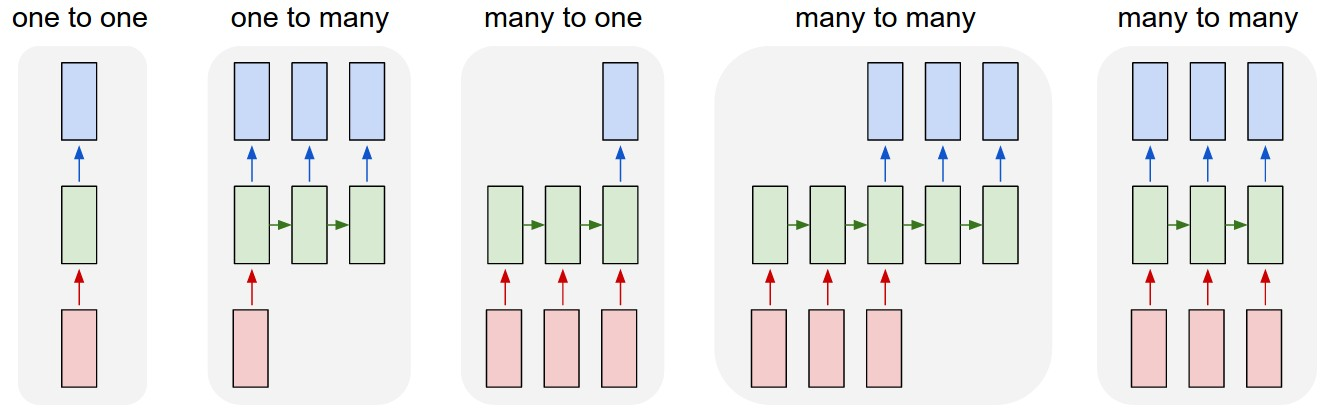
\includegraphics[width=100mm]{diagrams/rnn.jpeg}
	\caption{Rectangles represent vectors, with red being the input, blue the output, and green representing the state of the RNNs. Arrows represent  functions. From left to right: (1) an MLP. (2,3,4,5) are examples of different styles of recurrent neural networks, describing the different types of input and output combinations. (Diagram from \cite{karpathy_unreasonable_2015}) \label{rnn}} 
  \end{figure}
  
The architecture of RNNs make it favourable in NLP related problems as words in sentences are typically conditioned on the previous words. Given a sequence of inputs $(x_1, ..., x_M)$, a standard RNN computes a sequence of outputs $(y_1, ..., y_N)$ by performing forward-propagation in a similar to fashion to MLPs, but outputs are chained together as an additional input to other neural networks. This can be visualised best in Figure \ref{rnn}. RNNs are trained using backpropagation-through-time.

% talk about how much has been done with RNNs

RNNs showed promise but there existed a multitude of problems. Firstly, It became aparrent that it was very difficult for RNNs to leverage relationships between potentially relevant inputs and outputs - there isn't necessarily a clear indicator in the architecture that would facilitate this feature. This is described as a long range dependency problem. Furthermore, they were especially impractical due to the vanishing and exploding gradient problems having a larger effect on training. This is by design, as the architecture of the network does not provide the affordance to represent relationships between arbitary cells in the network.

\subsection{LSTMs and GRUs} 

Both gates were introduced to circumvent the issue of long range dependency problems by providing multiple avenues, with each one having a different approach.

\begin{figure}[!ht]
	\centering
	\begin{tikzpicture}[
		prod/.style={circle, draw, inner sep=0pt},
		ct/.style={circle, draw, inner sep=5pt, ultra thick, minimum width=10mm},
		ft/.style={circle, draw, minimum width=8mm, inner sep=1pt},
		filter/.style={circle, draw, minimum width=7mm, inner sep=1pt, path picture={\draw[thick, rounded corners] (path picture bounding box.center)--++(65:2mm)--++(0:1mm);
		\draw[thick, rounded corners] (path picture bounding box.center)--++(245:2mm)--++(180:1mm);}},
		mylabel/.style={font=\scriptsize\sffamily},
		>=LaTeX
		]
	
	\node[ct, label={[mylabel]Cell}] (ct) {$c_t$};
	\node[filter, right=of ct] (int1) {};
	\node[prod, right=of int1] (x1) {$\times$}; 
	\node[right=of x1] (ht) {$h_t$};
	\node[prod, left=of ct] (x2) {$\times$}; 
	\node[filter, left=of x2] (int2) {};
	\node[prod, below=5mm of ct] (x3) {$\times$}; 
	\node[ft, below=5mm of x3, label={[mylabel]right:Forget Gate}] (ft) {$f_t$};
	\node[ft, above=of x2, label={[mylabel]left:Input Gate}] (it) {$i_t$};
	\node[ft, above=of x1, label={[mylabel]left:Output Gate}] (ot) {$o_t$};
	
	\foreach \i/\j in {int2/x2, x2/ct, ct/int1, int1/x1,
				x1/ht, it/x2, ct/it, ct/ot, ot/x1, ft/x3}
		\draw[->] (\i)--(\j);
	
	\draw[->] (ct) to[bend right=45] (ft);
	
	\draw[->] (ct) to[bend right=30] (x3);
	\draw[->] (x3) to[bend right=30] (ct);
	
	\node[fit=(int2) (it) (ot) (ft), draw, inner sep=0pt] (fit) {};
	
	\draw[<-] (fit.west|-int2) coordinate (aux)--++(180:7mm) node[left]{$x_t$};
	\draw[<-] ([yshift=1mm]aux)--++(135:7mm);
	\draw[<-] ([yshift=-1mm]aux)--++(-135:7mm);
	
	\draw[<-] (fit.north-|it) coordinate (aux)--++(90:7mm) node[above]{$x_t$};
	\draw[<-] ([xshift=1mm]aux)--++(45:7mm);
	\draw[<-] ([xshift=-1mm]aux)--++(135:7mm);
	
	\draw[<-] (fit.north-|ot) coordinate (aux)--++(90:7mm) node[above]{$x_t$};
	\draw[<-] ([xshift=1mm]aux)--++(45:7mm);
	\draw[<-] ([xshift=-1mm]aux)--++(135:7mm);
	
	\draw[<-] (fit.south-|ft) coordinate (aux)--++(-90:7mm) node[below]{$x_t$};
	\draw[<-] ([xshift=1mm]aux)--++(-45:7mm);
	\draw[<-] ([xshift=-1mm]aux)--++(-135:7mm);
	\end{tikzpicture}
	\caption{A diagram of the LSTM model.}
\end{figure}
 
LSTM (Long Short Term Memory) is a type of RNN unit that attempts to retain information based on the previous inputs through the introduction of gated architectures. XXXXXXX

Introduced by \cite{cho_properties_2014}, GRUs are used to solve the common issue with LSTMs where the training time was relatively slow due to the number of derivatives necessary to compute. Within the GRU architecture, a feature to retain the previous weights remain, but there exists an direct path to the input data from the output, allowing a reduction in training time. They are unable to clearly distinguish between the performance of the two gated units they tested.
However, Some research from \cite{chung_empirical_2014} suggests that GRUs were found to perform better than LSTMs on smaller datasets. 

\section{Autoencoders}

Autoencoders are a specialised form of MLPs where the model attempts to recreate the inputs on the output. Autoencoders typically have a neural network layer in the model where its dimension is smaller than the input space, therefore representing a dimensionality reduction in the data. Autoencoders are composed of two different principal components, an encoder network $\alpha$ and a decoder network $\beta$, such that $\alpha : X \rightarrow F$ and $\beta : F \rightarrow X$. Measuring the success of the reconstruction is deduced by a reconstruction loss formula. This reconstruction loss comapres the output of the decoder and compares it against the input of the encoder. The two networks are trained together in a manner that allows them to preserve the input as much as possible.
% definitely need a diagram for autoencoders
% what is it good for?

Autoencoders are popularised through their use in Machine Translation, Word Embeddings, and document clustering.

% talk about how important this is in the context of the task.

\subsection{Measuring Performance}

"Bleu measures precision: how much the words (and/or n-grams) in the machine generated summaries appeared in the human reference summaries.

Rouge measures recall: how much the words (and/or n-grams) in the human reference summaries appeared in the machine generated summaries.

Naturally - these results are complementing, as is often the case in precision vs recall. If you have many words from the system results appearing in the human references you will have high Bleu, and if you have many words from the human references appearing in the system results you will have high Rouge."

% https://stackoverflow.com/questions/38045290/text-summarization-evaluation-bleu-vs-rouge

% http://opennmt.net OPENMNT-Py has BLEU/ROUGE on it.

\section{Related Work}


\subsection{Seq2Seq}

Seq2Seq, introduced by \cite{sutskever_sequence_2014} is a type of neural architecture that models relationships between sequences. In our particular scenario, this could be seen as a modern interpretation of the autoencoder. Seq2Seq comprises of two layers - Encoders and Decoders - which are both are represented with RNNs. This allows the architecture to take in arbitarily sized vectors, and allowing it to output similarly arbitary sized vectors. This flexibility makes it especially adventageous to NLP related problems.

\begin{figure}[!ht]
      
	\centering
	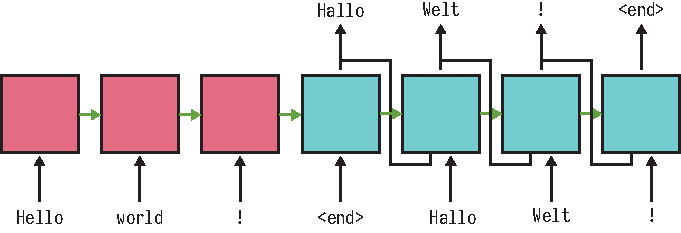
\includegraphics[width=100mm]{diagrams/seq2seq.pdf}
	\caption{An abstracted model of the seq2seq architecture, where the encoder (pink) takes in the input sequence, and the decoder (blue) shows the output sequence.\label{seq2seq}}
  \end{figure}

/ something good about seq2seq.

Traditionally, Seq2seq would be the most common method of tackling this particular problem, but it also presents problems that make it suboptimal. Seq2seq models have shown to be effective in reponse generation, but XXXXX

% fix this sentence. why is there lack of variabiity?
% but \cite{serban_hierarchical_2016}; \cite{zhao_learning_2017} suggest that one of the primary causes of the lack of variability of responses could be boiled down to the lack of model variability.
% why? remaining certain patterns?

Furthermore, it was discussed by \cite{jiang_why_2018} on the lack of diversity in responses. something something.

\subsection{Seq2Seq with Attention}

/ need diagram

Further work by \cite{bahdanau_neural_2014} improved the original seq2seq model by providing an attention mechanism. The attention mechanism looks at all of the inputs from the hidden states of the encoders so far. This allows the decoder network to "attend" to different parts of the source input at each step of the output generation. This circumvents the need to encode the full source input into a fixed-length vector, helping it deal with long-range dependency problems.

% fix this section
Furthermore, this attention mechanism allows the model to learn what to attend to based on the input sequence and what it has so far, represented through a weighted combination of the two. \cite{bahdanau_neural_2014} have found this to work especially well in machine translation problems where languages which are relatively well aligned (such as English and German) - The decoder is most likely able to choose to attend to the response generation sequentially, such that the first output from the decoder can be generated based on the properties of the first input of the encoder and so on.

% mention the limitations of Seq2seq for your problem and ways they could be addressed (VAEs, etc.), describe the VAE approach and your motivation to pick it, introduce the VAE paper you work with in details.

\subsection{Transformers}

\begin{figure}[!ht]
      
	\centering
	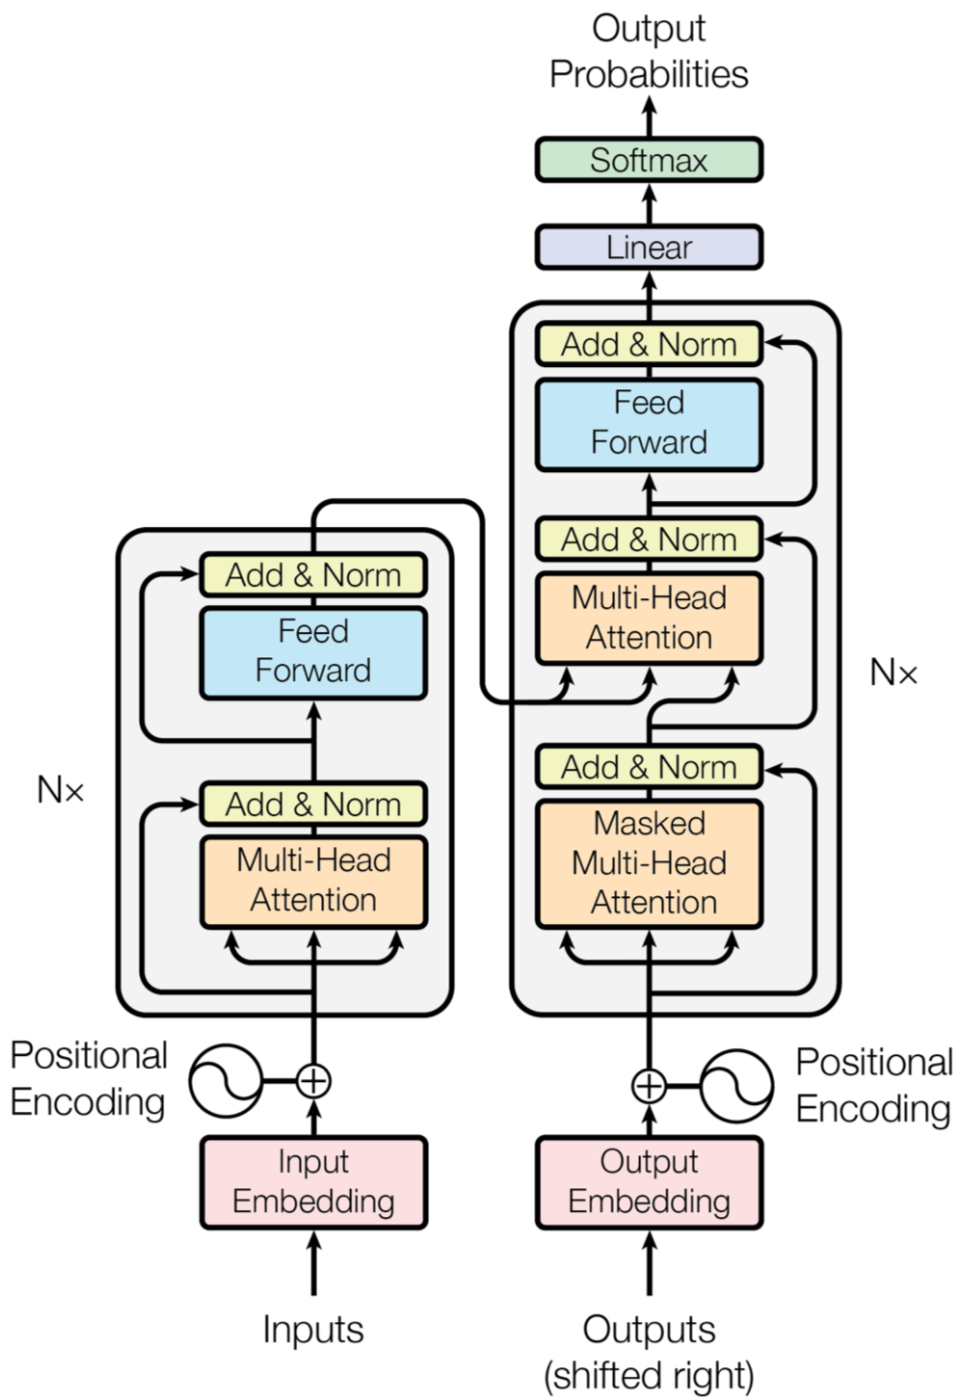
\includegraphics[width=60mm]{diagrams/transformers.png}
	\caption{The transformer model architecture.\cite{vaswani_attention_2017} \label{transformer}}
  \end{figure}

\cite{vaswani_attention_2017} introduced the idea that it is possible to avoid the use of RNNs altogether and focus on leveraging the attention mechanism introduced in seq2seq. The resulting network architecture utilises stacked layers of residual networks for the encoder and the decoder.

% talk about multihead attention

% taalk about removing recursion/recurrentness of the network
% mention that this will be used as the baseline
% "for text generation techniques, we will use this as the baseline"

\section{Variational Autoencoders}

Our proposed solution revolves around the use of Variational Autoencoders. Variational Autoencoders (VAEs) introduce a constraint on the encoding network that forces the model to generate latent vectors that roughly follow a gaussian distribution, as opposed to creating a fixed latent vector. Consequently, VAEs introduce two extra vectors, a mean vector and a standard distribution vector, which is fed from the encoder. A sample is taken from the distribution and that is then fed into the decoder.

\begin{figure}[!ht]
      
	\centering
	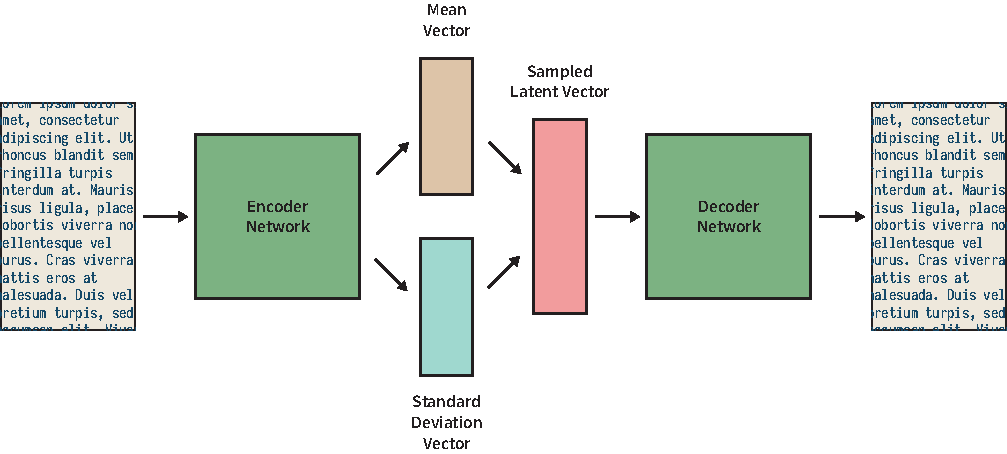
\includegraphics[width=150mm]{diagrams/variational_autoencoders.pdf}
	\caption{A simplified model architecture for a variational autoencoder, which takes as input some text, and it's predicted output being the same text as the input.\label{vae}}
  \end{figure}

  Note that the decoder receives samples from a non-standard normal distribution produced by the encoder. The average of the samples of the different distributions should approximate to a standard normal. This stochasticity allows us to model variability in the results. 
  
  Due to the stochastic nature of the network, we use a reconstruction loss that involves an expection of the output; but we also use the KL divergence, which  measures the relative difference of two probability distributions. In this particular case, we will be comparing the distribution of the decoder outputs against a standard gaussian $ \mathcal{N}(0,1)$).
  
  $$\mathcal{L}(\theta, \phi, x, z) = \mathbb{E}_{q \phi (z|x)}[log \thinspace p_{\theta}(x|z)] - D_{KL}(q_{\phi}(z|x)\thinspace||\thinspace p(z)) $$

$$
D_{KL}(P ||Q) = \sum_{x \subset X} P(x) \cdot log (\frac{P(x)}{Q(x)})
$$

In other words, it is the expectation of the logarithmic difference between the probabilities $P$ and $Q$, where the expectation of $P$ is already known.

\subsection*{Reparameterisation Trick}
- You'll need to perform a reparameterisation trick (since you can't calculate derivatives of samples.) in order to perform backpropagation. (you can't push gradients through a sampling node.)
  
$$z = \mu + \sigma \cdot \epsilon $$ where $\epsilon \sim \mathcal{N}(0,1)$. You want to learn $\mu, \sigma$.

\subsection{Conditional Variational Autoencoders}

Although VAEs are more robust when compared to their original autoencoder counterparts, the decoder class cannot produce outputs of a particular class on demand. CVAEs are an improved model of the original VAE architecture by conditioning on another description of the data, a class descriptor $y$. 

\begin{figure}[!ht]
      
	\centering
	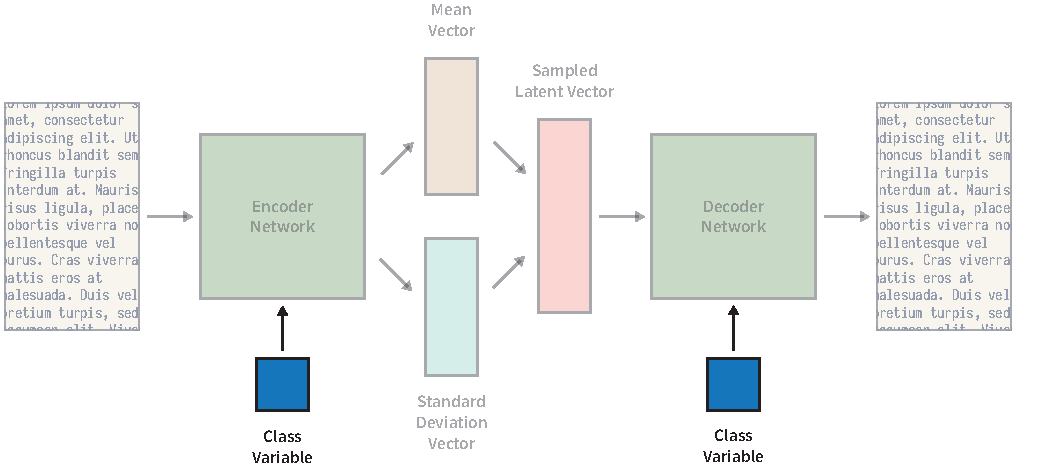
\includegraphics[width=150mm]{diagrams/conditional_variational_autoencoders.pdf}
	\caption{A model architecture for a CVAE, which includes the label being fed into the encoder and decoder networks. \label{cvae_diagram}}
  \end{figure}

During training time, a class (represented by some arbitary vector) is fed at the same time to the encoder and decoder. To generate an output that depends on $y$ we feed that number to the decoder along with a random point in the latent space sampled from a standard normal distribution.

Samples can be generated from the conditional distribution $p(x|y)$. By changing the value of $y$, we can get corresponding samples $x \sim p(x|y)$. The system no longer relies on the latent space to encode what output is necessary; instead the latent space encodes other information that can distinguish itself based on the differing $y$ values.

% However, it was found by \cite{du_variational_2018} that since the responses were generated from the same latent variable (induced by the class), it was difficult to model high-variability in responses.

% That being said, using this model alone is not sufficent. If we train the dataset on a vanilla VAE, assuming that the dataset can be encapsulated and modelled in such a manner that allows it to be processed in the model, outputs from the VAE alone will only produce some latent representive of the mean of the training data. 

\section{Variational Autoregressive Decoders}

To increase variability of outcomes produced by the original seq2seq model, \cite{serban_hierarchical_2016}; \cite{zhao_learning_2017} proposed the use of variational autoencoders to seq2seq models. At generation time, the latent variable $z$ can be used as a conditional signal of the decoder in the seq2seq model. Although this introduces variability in the outputs, the variability is not controlled; i.e it is produced from the randomness of $z$. The underlying seq2seq model remains suboptimal.

Introduced by \cite{du_variational_2018}, Variational Autoregressive Decoders (VADs) attempt to circumvent the sampling problem introduced from CVAEs by introducing multiple latent variables into the autoregressive Decoder. At different time-steps, this allows the decoder to produce a multimodal distribution of text sequences, allowing a variety of responses to be produced. 

We will be using this model to help solve the variability of outcomes. *WHY?*

VADs use the seq2seq architecture as the base with variable-length queries $x = \{x_1, x_2, ..., x_n\}$, and $y = \{y_1, y_2, ..., y_n\}$ representing the input and output responses respectively. The encoder network is a Bidirectional RNN with GRUs. The decoder network is an unidirectional RNN with GRUs. For each timestep $t$, each GRU in the decoder network is encoded with hidden state $h^d_t$.

\subsubsection{Sequential Model}

- uses a backwards RNN that represents the actual response to better create a posterior distribution.

\subsubsection{Prior Model}

a simple neural net that produces an output that represents a conditional variable for our output generation.

\subsubsection{Auxillary Objective}

An auxillary objective that attempts to predict the bag of words based on the latent variable. Helps to improve the output options.

\subsubsection{Learning Mechanism}

VADs use a weighted combination of ELBO and the log likelihood loss of the auxillary objective.



% %%%%%%%%%%%%%%%%%%%%%%%%%%%%%%%%%%%%
% \chapter{Contribution}


% %%%%%%%%%%%%%%%%%%%%%%%%%%%%%%%%%%%%
% \chapter{Experimental Results}


% %%%%%%%%%%%%%%%%%%%%%%%%%%%%%%%%%%%%
% \chapter{Conclusion}


%% bibliography
\bibliographystyle{apa}
\bibliography{ref} 

\end{document}
